\documentclass[11pt,a4paper]{article}

\usepackage[margin=24mm]{geometry}
\usepackage[T1]{fontenc}
\usepackage[utf8]{inputenc}
\usepackage{lmodern}
\usepackage{microtype}
\usepackage{amsmath,amssymb}
\usepackage{booktabs,longtable,array}
\usepackage{graphicx}
\usepackage{float}
\usepackage{xcolor}
\usepackage{siunitx}
\usepackage{enumitem}
\usepackage{hyperref}

\hypersetup{
  colorlinks=true,
  linkcolor=blue!55!black,
  urlcolor=blue!65!black,
  citecolor=blue!55!black,
  pdftitle={Five-mirror EUV projection-optics simulator},
  pdfauthor={Project documentation}
}
\sisetup{per-mode=symbol,detect-all=true}
\graphicspath{{figures/}}
\setlist{nosep}

\newcommand{\notebook}{\path{five_mirror_EUV_projection_simulation.ipynb}}
\newcommand{\plotorplaceholder}[1]{%
  \IfFileExists{figures/#1.pdf}{%
    \includegraphics[width=\linewidth]{figures/#1.pdf}%
  }{%
    \IfFileExists{figures/#1.png}{%
      \includegraphics[width=\linewidth]{figures/#1.png}%
    }{%
      \fbox{\parbox[c][55mm][c]{0.94\linewidth}{\centering
        Figure not exported yet. Restart the Jupyter kernel and run all cells in
        \notebook. The notebook will create \path{figures/#1.pdf}.}}%
    }%
  }%
}

\title{Five-Mirror EUV Projection-Optics Simulator at \SI{13.5}{nm}}
\author{Generated for the Mirrors in EUV project}
\date{\today}

\begin{document}
\maketitle


\section{Purpose and scope}

This document describes the numerical setup, editable mirror and coating
parameters, exported data, and every non-interactive plot produced by
\notebook.  The model is intended as an inspectable research and teaching
starting point for studying five reflective projection surfaces at the
\SI{13.5}{nm} wavelength used in extreme-ultraviolet (EUV) lithography.

The notebook deliberately separates two physical calculations:

\begin{enumerate}
  \item \textbf{Geometrical propagation.} Optiland traces rays through five
  rotationally symmetric reflective aspheres and onto a wafer plane.  This
  part determines ray intercepts, field mapping, aberration-induced spot
  shape, and sensitivity to curvature or aspheric figure.

  \item \textbf{Multilayer reflection.} A NumPy transfer-matrix calculation
  evaluates a vacuum/Ru/(Si/Mo)$_{40}$/ substrate stack.  This part determines
  reflected power versus wavelength, incidence angle, polarization, coating
  thickness, pair count, and interface roughness.  Coating loss weights the
  rays but does not alter their directions in this notebook.
\end{enumerate}

\section{Optical setup}

\subsection{Overall Structure of Mirrors}
\begin{figure}[H]
\centering
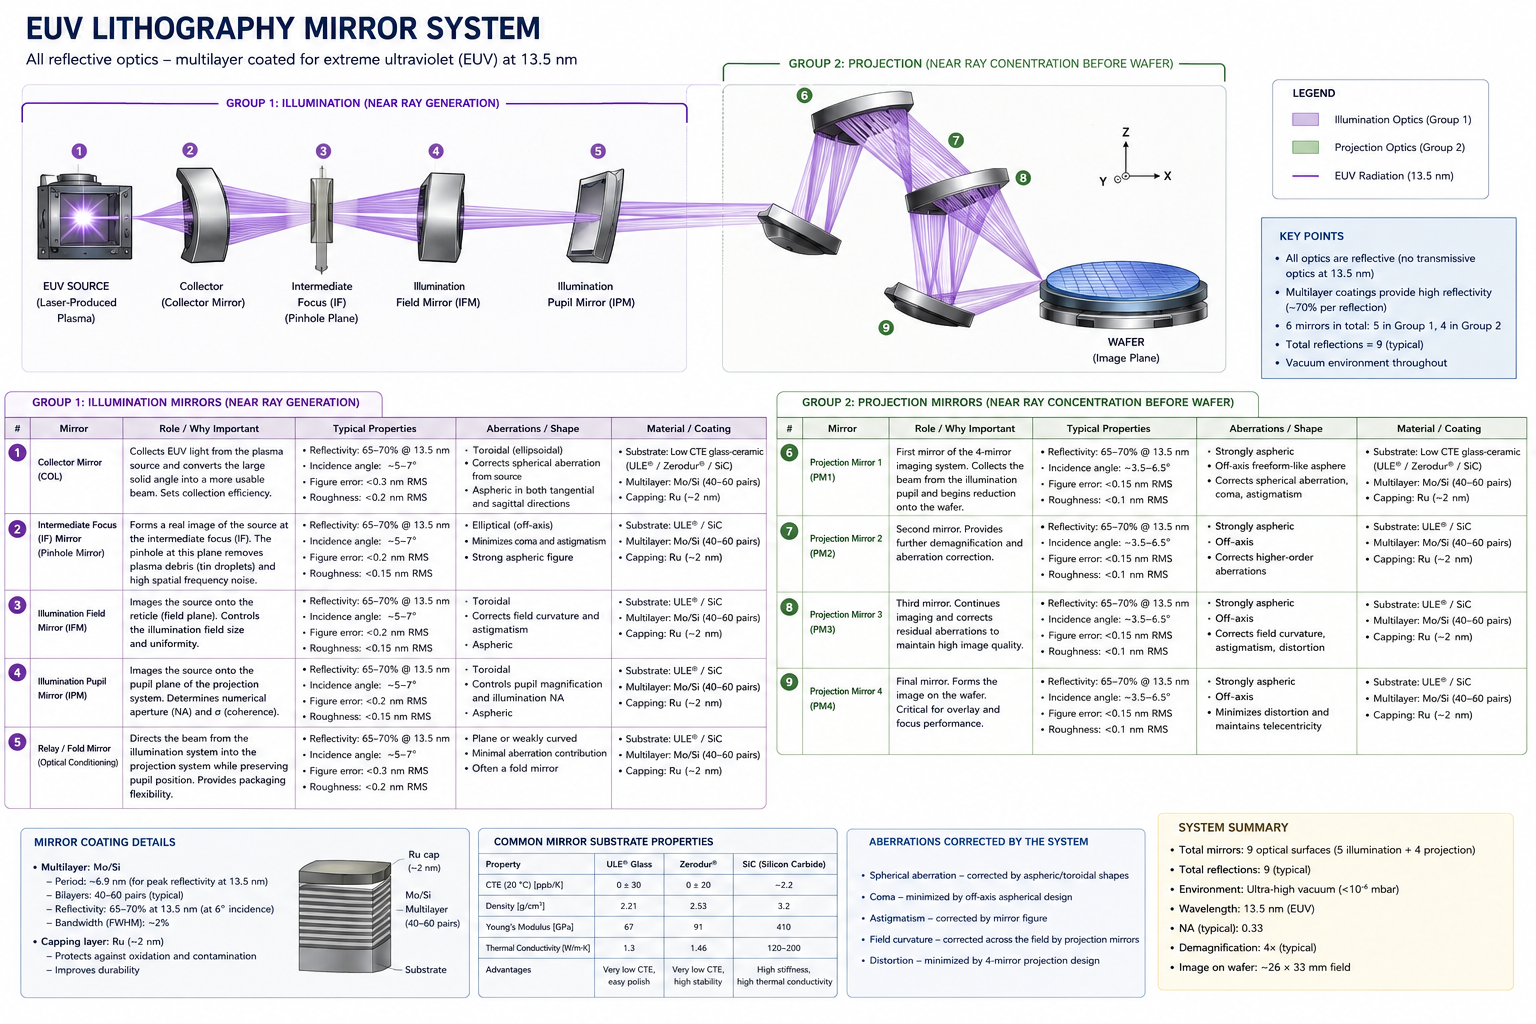
\includegraphics[width = \linewidth]{Mirrors Illustration.png}
\caption{Setup of the two sets of Mirrors in a photo-lithography machine}
\end{figure}


\subsection{Global settings and units}

Table~\ref{tab:global} summarizes the nominal global configuration.  Optiland
uses millimetres for spatial coordinates and micrometres for wavelength;
therefore the notebook passes \SI{13.5}{nm} as \SI{0.0135}{\micro\metre}.  The
coating solver uses nanometres for wavelength, film thickness, and roughness.

\begin{table}[H]
\centering
\caption{Global simulation settings.}
\label{tab:global}
\begin{tabular}{@{}lll@{}}
\toprule
Quantity & Nominal value & Meaning \\
\midrule
Wavelength & \SI{13.5}{nm} & Monochromatic EUV ray-trace wavelength \\
Object distance & \SI{351.141510}{mm} & Mask plane to M1 vertex \\
Image-space f-number & 2.78 & Aperture specification \\
Mask-field heights & $-208,-211,-214$ mm & Three samples across the ring field \\
Stop surface & M4 & Physically accessible aperture stop \\
Random seed & 7 & Repeatable random-pupil spot sampling \\
\bottomrule
\end{tabular}
\end{table}

The system is surface-sequential.  A surface's ``thickness to next'' is the
signed axial distance from that surface vertex to the next surface vertex in
the current propagation direction.  Because a mirror reverses propagation,
the signs alternate through the folded sequence.  These negative spacings are
therefore intentional; replacing them by absolute values does not merely move
a component but changes the optical path topology.

The mask samples lie near the centre of the disclosed annular field.  In calls
to \texttt{system.trace}, $H_y=-1,0,+1$ are \emph{normalized field
coordinates}; they select the two field endpoints and the central field.  They
are not millimetre coordinates.  The corresponding physical mask heights are
specified by \path{FIELD_Y_MM}, while the actual image-plane intercepts are
exported in millimetres.

\subsection{Five-mirror prescription}

The default geometry is based on the public five-mirror, 4:1 reduction,
NA~0.18 prescription in US6072852A.  Its power sequence is concave--convex--
concave--convex--concave.  Table~\ref{tab:mirrors} lists the values entered in
the notebook.  Radius is the vertex radius of the base conic.  A negative
radius follows the patent/Optiland sequential sign convention; it should not
be interpreted without the signed spacing and current propagation direction.

\begin{table}[H]
\centering
\caption{Nominal mirror settings. AOI is measured from the surface normal.}
\label{tab:mirrors}
\small
\begin{tabular}{@{}lrrrrrl@{}}
\toprule
Mirror & Radius (mm) & To next (mm) & $K$ & AOI (deg) & AOI half-span (deg) & Role \\
\midrule
M1 & -1277.318653 & -292.381122 & 1.626111 & 11.34 & 2.0 & Concave power \\
M2 &  -417.634186 &  504.794891 & 0.339465 &  7.72 & 2.0 & Convex power \\
M3 &  -757.329052 & -496.445439 & 0.026174 &  5.28 & 2.0 & Concave power \\
M4 &  -448.096932 &  193.582965 & 2.592761 & 15.52 & 3.0 & Convex power; stop \\
M5 &  -392.026187 & -260.692804 & 0.346595 &  7.76 & 2.0 & Concave power \\
\bottomrule
\end{tabular}
\end{table}

The AOI half-span is used only by the approximate pupil-apodization plot.  It
represents a linear engineering estimate of angle variation across each beam
footprint, not a recovered local-angle map from the patent.  Changing this
number modifies the pupil-intensity estimate but not the Optiland ray path.

Every default surface is an even asphere with sag
\begin{equation}
 z(r)=\frac{c r^2}{1+\sqrt{1-(1+K)c^2r^2}}
      +A r^4+B r^6+C r^8+D r^{10},
 \qquad c=\frac{1}{R}.
 \label{eq:sag}
\end{equation}
Optiland stores an even-asphere coefficient vector beginning at $r^2$, so the
notebook passes $[0,A,B,C,D]$.  Table~\ref{tab:aspheres} lists the deformation
coefficients.  Their dimensions are those needed for $z$ and $r$ in
millimetres: $A$ has units mm$^{-3}$, $B$ mm$^{-5}$, $C$ mm$^{-7}$, and $D$
mm$^{-9}$.

\begin{table}[H]
\centering
\caption{Even-asphere deformation coefficients in Equation~\eqref{eq:sag}.}
\label{tab:aspheres}
\small
\begin{tabular}{@{}lrrrr@{}}
\toprule
Mirror & $A$ & $B$ & $C$ & $D$ \\
\midrule
M1 & 0 & $ 3.498200\times10^{-16}$ & $-7.101160\times10^{-22}$ & 0 \\
M2 & 0 & $ 5.759030\times10^{-15}$ & $ 9.512560\times10^{-20}$ & 0 \\
M3 & 0 & $ 1.143970\times10^{-17}$ & $ 7.746320\times10^{-23}$ & 0 \\
M4 & 0 & $-9.009250\times10^{-15}$ & $-2.722770\times10^{-19}$ & 0 \\
M5 & 0 & $-9.701720\times10^{-16}$ & $-1.567560\times10^{-20}$ & 0 \\
\bottomrule
\end{tabular}
\end{table}

The editable mirror dictionaries also expose clear-aperture radius, $x/y$
decenter, and $x/y$ tilt.  Aperture radius is left as \texttt{None} by default,
allowing Optiland to establish the working semi-apertures from the f-number and
stop.  Tilts are in radians; radii, spacings, and decentres are in millimetres.

\section{Mo/Si multilayer and Ru cap}

\subsection{Layer sequence}

Each mirror has an independent coating dictionary.  From the incident vacuum
toward the substrate, the nominal stack is
\begin{equation}
 \text{vacuum}/\mathrm{Ru}(1.50\,nm)/
 [\mathrm{Si}(4.15\,nm)/\mathrm{Mo}(2.80\,nm)]_{40}/\text{substrate}.
\end{equation}
The nominal bilayer period is therefore \SI{6.95}{nm}.  The dictionary permits
different Mo, Si, and Ru thicknesses on every mirror, different pair counts,
linear depth grading, and arbitrary individual-layer overrides.  Individual
layers are named from the vacuum side, for example \texttt{Si\_01},
\texttt{Mo\_01}, and \texttt{Mo\_40}.  The files
\path{data/layer_stack_M1.csv} through
\path{data/layer_stack_M5.csv} record the fully expanded stack actually used.

The reference complex indices at \SI{13.5}{nm} are shown in
Table~\ref{tab:indices}.  The notebook uses the passive convention
$\tilde n=n+ik$ with $k>0$ and a propagation phase that decays in absorbing
media.

\begin{table}[H]
\centering
\caption{Reference complex refractive indices at \SI{13.5}{nm}.}
\label{tab:indices}
\begin{tabular}{@{}lrr@{}}
\toprule
Material & $n$ & $k$ \\
\midrule
Vacuum & 1.000000000 & 0 \\
Ru & 0.886360034 & 0.017064894 \\
Si & 0.999002305 & 0.001826494 \\
Mo & 0.923793525 & 0.006435425 \\
Effective substrate & 0.973713000 & 0.012976400 \\
\bottomrule
\end{tabular}
\end{table}

These indices are held constant over the narrow \SIrange{12.5}{14.5}{nm}
plotting interval.  Consequently, the plotted wavelength sensitivity captures
the interference-phase and thickness effects cleanly, but it is not a
substitute for a measured dispersive $n(\lambda)+ik(\lambda)$ dataset when
absolute broadband accuracy is required.

\subsection{Reflectivity calculation}

For incident angle $\theta_0$, Snell's law is applied in complex form to each
layer $j$,
\begin{equation}
 \cos\theta_j=\sqrt{1-\left(\frac{n_0\sin\theta_0}{n_j}\right)^2},
 \qquad k_{z,j}=\frac{2\pi}{\lambda}n_j\cos\theta_j,
\end{equation}
with the square-root branch selected to give passive propagation.  The optical
admittances are $q_j^{(s)}=n_j\cos\theta_j$ and
$q_j^{(p)}=\cos\theta_j/n_j$.  The interface amplitude is
\begin{equation}
 r_{ij}=\frac{q_i-q_j}{q_i+q_j}.
\end{equation}
The recursion combines every interface amplitude with the round-trip layer
phase $\exp(2ik_{z,j}d_j)$.  A compact Nevot--Croce-like factor
\begin{equation}
 \exp\!\left[-2\left|k_{z,i}k_{z,j}\right|\sigma^2\right]
\end{equation}
reduces each interface amplitude for nominal RMS roughness
$\sigma=\SI{0.25}{nm}$.  This term is intentionally approximate: it does not
distinguish topographic roughness from interdiffusion or silicide formation.
The unpolarized power reflectivity is
$R=(|r_s|^2+|r_p|^2)/2$.

\section{Plots and Interpretations}

\subsection{Mirror reflectivity and cumulative intensity}

\begin{figure}[H]
\centering
\plotorplaceholder{01_mirror_reflectivity_and_cumulative_intensity}
\caption{Individual multilayer reflectivity (left) and cumulative five-mirror
intensity (right).}
\label{fig:spectrum}
\end{figure}

\paragraph{Left-panel axes.}
The horizontal axis is vacuum wavelength in nanometres, from
\SIrange{12.5}{14.5}{nm}.  The dashed vertical line marks the operating
wavelength, \SI{13.5}{nm}.  The vertical axis is reflected optical power as a
percentage of the power incident on the particular mirror.  Each coloured
curve uses that mirror's own nominal AOI and coating dictionary.  Curves can
differ even when their physical layer thicknesses are identical because the
normal component of wavevector and hence the Bragg condition change with AOI.

\paragraph{Right-panel axes.}
The horizontal axis and dashed reference line have the same meanings.  The
vertical axis is power remaining relative to the power entering M1.  The curve
labelled ``after M$n$'' is
\begin{equation}
 I_n(\lambda)/I_0=\prod_{j=1}^{n}R_j(\lambda).
\end{equation}
The curves must therefore move downward as more mirrors are included.  This
multiplicative loss is why a few percentage points of reflectivity improvement
per surface can materially change total scanner throughput.  The exported
\path{data/reflectivity_spectrum.csv} stores wavelength, every individual
reflectivity as a fraction, and every cumulative fraction.  Percent values in
the plot are 100 times those fractions.

At the dashed \SI{13.5}{nm} line, the present default calculation gives
$R_1=53.10\%$, $R_2=71.84\%$, $R_3=73.03\%$, $R_4=12.50\%$, and
$R_5=71.79\%$.  Their product is only $2.501\%$.  M4 is the dominant loss in
this particular baseline because it has the largest nominal AOI
(\SI{15.52}{\degree}) while all five mirrors initially share one ungraded
stack.  This should be interpreted as a coating-tuning result, not as an
intrinsic inability of a five-mirror system to transmit more power.  A
per-mirror stack optimized for M4's AOI would shift its Bragg maximum toward
\SI{13.5}{nm} and materially improve the product.

Changing Mo or Si thickness primarily translates and reshapes the Bragg peak;
changing pair count changes peak build-up and bandwidth; increasing roughness
usually lowers peak reflectivity; and changing the Ru cap affects both
absorption and the phase presented to the periodic stack.

\subsection{Estimated coating apodization across the pupil}

\begin{figure}[H]
\centering
\plotorplaceholder{02_pupil_apodization}
\caption{Estimated cumulative coating intensity across a normalized pupil
diameter at \SI{13.5}{nm}.}
\label{fig:pupil}
\end{figure}

The horizontal axis is a dimensionless normalized pupil coordinate $p$.
$p=-1$ and $p=+1$ are opposite edges of the sampled pupil diameter, while
$p=0$ is its centre.  It is not a millimetre coordinate on any one mirror.
For mirror $j$, the notebook assigns
\begin{equation}
 \theta_j(p)=\bar\theta_j+\Delta\theta_j p,
\end{equation}
where $\bar\theta_j$ is the nominal AOI and $\Delta\theta_j$ is the editable
half-span in Table~\ref{tab:mirrors}.  The vertical axis is cumulative power
relative to the power entering M1, expressed in percent.  Each curve again
adds one mirror to the product, now evaluated at a pupil-dependent AOI.

Slope or asymmetry in these curves represents coating-induced pupil
apodization: different parts of the pupil reach the wafer with different
amplitudes.  Such amplitude variation can alter the effective pupil and, in a
wave-optical model, the point-spread function and imaging contrast.  The plot
is a sensitivity estimate, not a rigorous coating map, because the assumed AOI
variation is linear and one-dimensional.  The CSV
\path{data/pupil_apodization.csv} includes $p$, local AOI, individual
reflectivity, and cumulative intensity after each mirror.

The asymmetry is large for the current common-stack example.  The final
five-mirror fraction is approximately $7.79\%$ at $p=-1$, $2.501\%$ at
$p=0$, and $0.0717\%$ at $p=+1$.  The collapse toward $p=+1$ follows the
assumed increase in AOI and the strong off-Bragg response of M4.  Because the
AOI half-spans are illustrative rather than extracted from local ray normals,
these endpoint values are best used to compare coating choices, not as a
certified scanner pupil-uniformity prediction.

\subsection{Optiland meridional ray diagram}

\begin{figure}[H]
\centering
\plotorplaceholder{03_optiland_ray_diagram}
\caption{Sequential Optiland ray diagram for the five reflective aspheres and
three mask-field samples at \SI{13.5}{nm}.}
\label{fig:rays}
\end{figure}

The horizontal axis is Optiland global $Z$ in millimetres.  It is the
meridional layout direction and should not be confused with propagation
distance accumulated along a ray.  Because the path folds at every reflection,
a later surface in sequential order can have a smaller global $Z$ coordinate.
The vertical axis is global meridional height $Y$ in millimetres.  It shows the
off-axis ring field, mirror footprints, and convergence or divergence of the
sampled ray bundles.  The plotted lines are geometrical rays; their separation
is a pupil-sampling choice and is not an intensity scale.  Surface arcs show
the local conic/aspheric profiles over their working apertures.  M4 is the stop
and therefore determines the accepted bundle in conjunction with the
image-space f-number.

This plot should be read topologically: follow each ray in surface order
mask--M1--M2--M3--M4--M5--wafer rather than assuming monotonically increasing
$Z$.  A blank or discontinuous bundle after parameter editing normally means
that rays miss a surface, encounter an invalid sag domain, or are vignetted by
an imposed aperture.  Restore the signed spacings before diagnosing smaller
curvature changes.

\subsection{Final wafer-plane ray shape}

\begin{figure}[H]
\centering
\plotorplaceholder{04_final_wafer_ray_shape}
\caption{Centred geometrical spot, weighted ray-density map, and three-field
wafer footprints.}
\label{fig:wafer}
\end{figure}

Figure~\ref{fig:wafer} contains three related views.

\paragraph{Left panel: centred middle-field spot.}
Both axes are image-plane displacement from the weighted middle-field centroid
in nanometres.  One plotted point is one surviving geometrical ray.  Equal
scales on the two axes preserve spot shape.  The title reports the weighted
RMS radius
\begin{equation}
 r_{\mathrm{RMS}}=
 \sqrt{\frac{\sum_i w_i[(x_i-\bar x)^2+(y_i-\bar y)^2]}{\sum_i w_i}},
\end{equation}
where $w_i$ includes Optiland ray intensity and the five-mirror coating
throughput.  Centring removes field position so that coma, astigmatism, and
other shape changes are visible.  It also hides absolute distortion, which is
why the right panel is required.

\paragraph{Middle panel: weighted ray-density shape.}
The horizontal and vertical axes are the same centred nanometre coordinates.
Colour represents the sum of relative deposited ray power within each
two-dimensional histogram bin.  A brighter bin contains more weighted rays;
the colour scale is relative, not calibrated irradiance in
W\,m$^{-2}$.  Monte Carlo granularity decreases as the number of traced rays is
increased.

\paragraph{Right panel: three physical field footprints.}
The axes are absolute image-plane $x$ and $y$ in millimetres.  Colours identify
normalized fields $H_y=-1,0,+1$.  Separation of the three groups shows field
mapping and magnification; displacement from ideal field positions indicates
distortion.  The millimetre scale is much larger than the nanometre centred
spot scale in the other panels, so individual aberration shapes can appear
compressed here.

Raw middle-field intercepts are in
\path{data/middle_field_spot.csv}; all three fields are in
\path{data/three_field_footprints.csv}; and throughput, valid-ray count, and
RMS radius are in \path{data/wafer_spot_metrics.csv}.  Coordinates in the CSV
remain in millimetres so no precision is lost through display-unit conversion.

For the recorded run, all 2500 middle-field rays reached the image plane.  The
reported geometrical RMS radius is \SI{3858.27}{nm}, or about
\SI{3.86}{\micro\metre}, and the coating weight is $2.501\%$.  The three
field centroids lie near image $y=+53.5003$, $0$, and $-53.5003$ mm for
$H_y=-1,0,+1$, respectively, consistent with the inverted ring-field mapping.
The centre field has a small mean $x$ offset of roughly
$-1.16\times10^{-4}$ mm in the finite Monte Carlo sample.  These numbers
describe this public starting prescription and sampling scheme; the micrometre-
scale geometrical spot is not a claim of production-lithography performance.

\subsection{M3 curvature sensitivity}

\begin{figure}[H]
\centering
\plotorplaceholder{05_geometry_sensitivity_m3}
\caption{Middle-field spot sensitivity to a $+0.02\%$ change in the M3 vertex
radius.}
\label{fig:sensitivity}
\end{figure}

The demonstration multiplies the M3 radius by 1.0002 while retaining its
conic, aspheric coefficients, spacing, and all other mirrors.  Both axes are
nanometres relative to the \emph{nominal} spot centroid.  The nominal and
changed clouds share one reference origin; therefore a changed-cloud offset is
a real image-centroid shift rather than an artefact removed by independently
centring the two cases.  A change in cloud width or shape indicates altered
aberration, while a mostly rigid translation indicates image displacement.

The comparison is a one-variable sensitivity experiment, not a tolerance
allocation.  A realistic tolerance study would vary radius, spacing, decenter,
tilt, low- and mid-spatial-frequency figure terms, and compensator settings,
then report distributions over many trials.  The plotted points and weights
are exported to \path{data/geometry_sensitivity_m3.csv}.  Calling the helper
for another mirror creates a correspondingly named CSV and figure, but those
additional user-generated plots are not automatically included in this README.

Numerically, the demonstration changes M3 from approximately
$-757.329052$ mm to $-757.480518$ mm.  The changed centroid moves by
\SI{244.59}{nm}.  With both cases measured about the nominal centroid, the
weighted RMS radius grows from approximately \SI{3.84}{\micro\metre} to
\SI{10.68}{\micro\metre}.  The orange cloud is therefore not merely translated:
its much larger extent shows a strong degradation of the nominal aberration
balance from a seemingly small $0.02\%$ radius perturbation.

% \section{Exported files and column meanings}

% \subsection{Figures}

% Each entry is written as both \texttt{.png} and \texttt{.pdf} in
% \path{figures/}:

% \begin{longtable}{@{}p{0.49\linewidth}p{0.45\linewidth}@{}}
% \toprule
% Stem & Contents \\
% \midrule
% \endhead
% \path{01_mirror_reflectivity_and_cumulative_intensity} & Individual and cumulative spectral power \\
% \path{02_pupil_apodization} & Approximate cumulative power versus normalized pupil \\
% \path{03_optiland_ray_diagram} & Five-mirror sequential meridional layout \\
% \path{04_final_wafer_ray_shape} & Centred spot, density, and three-field footprints \\
% \path{05_geometry_sensitivity_m3} & Nominal versus perturbed M3 ray intercepts \\
% \bottomrule
% \end{longtable}

% \subsection{Data}

% \begin{longtable}{@{}p{0.39\linewidth}p{0.56\linewidth}@{}}
% \toprule
% File & Interpretation \\
% \midrule
% \endhead
% \path{simulation_configuration.json} & Complete global, mirror, coating, field, and optical-index configuration \\
% \path{mirror_geometry.csv} & One row per mirror: radius, signed next spacing, conic, nominal AOI, and surface type \\
% \path{asphere_coefficients.csv} & One row per mirror containing the $r^4$, $r^6$, $r^8$, and $r^{10}$ coefficients with units encoded in the column names \\
% \path{optical_constants_13p5nm.csv} & Material, wavelength, real index, and extinction coefficient \\
% \path{layer_stack_M1.csv}--\path{layer_stack_M5.csv} & Expanded incident-side layer number, layer name, material, and thickness in nm \\
% \path{coating_summary_13p5nm.csv} & Per-mirror AOI, pair count, nominal material thicknesses, reflectivity percent, and cumulative percent \\
% \path{reflectivity_spectrum.csv} & Wavelength and individual/cumulative reflected-power fractions \\
% \path{pupil_apodization.csv} & Normalized pupil, local AOIs, individual fractions, and cumulative fractions \\
% \path{ray_diagram_intercepts.csv} & Normalized field, sequential surface and ray indices, and global $x,y,z$ intercepts in mm \\
% \path{middle_field_spot.csv} & Final $x,y$ intercepts in mm and relative ray power for $H_y=0$ \\
% \path{three_field_footprints.csv} & Normalized field identifier, final $x,y$ in mm, and relative ray power \\
% \path{wafer_spot_metrics.csv} & Wavelength, valid ray count, total throughput fraction, and RMS radius in nm \\
% \path{geometry_sensitivity_m3.csv} & Case label, $x,y$ relative to nominal centroid in nm, and ray power \\
% \bottomrule
% \end{longtable}

% Columns containing \texttt{fraction} range nominally from 0 to 1; multiply by
% 100 for percent.  Columns explicitly containing \texttt{percent} are already
% scaled.  A ``relative ray power'' is suitable for weighting and comparison but
% is not an absolute radiometric unit.

% \section{Recommended parameter-study procedure}

% To isolate causes and preserve reproducibility:

% \begin{enumerate}
%   \item Copy the baseline JSON and CSV exports before changing the notebook.
%   \item Change one parameter family at a time: coating thickness, roughness,
%   mirror radius, conic, higher-order asphere, spacing, or alignment.
%   \item Rerun from the editable configuration cell.  Geometry changes require
%   rebuilding the Optiland system; coating-only changes do not alter ray
%   coordinates in the present model.
%   \item Check Figure~\ref{fig:spectrum} first for coating resonance and total
%   throughput, Figure~\ref{fig:pupil} for amplitude uniformity, then
%   Figures~\ref{fig:rays}--\ref{fig:sensitivity} for ray-path validity and image
%   quality.
%   \item Archive the updated \path{simulation_configuration.json} with the
%   figures.  Without it, a plot is not a reproducible simulation result.
% \end{enumerate}

% For coating optimization, tune the Si/Mo period to place the reflectivity peak
% near \SI{13.5}{nm} at each mirror's AOI, then examine pair count, thickness
% ratio, Ru cap, roughness, bandwidth, and pupil variation.  For geometry
% sensitivity, begin with relative radius changes of order $10^{-5}$--$10^{-4}$
% and small conic/asphere perturbations.  Large edits often invalidate the
% sequential path before yielding an interpretable sensitivity.

% \section{Limitations and responsible interpretation}

% \begin{itemize}
%   \item The public prescription is an older five-mirror design originally
%   associated with approximately \SI{13.1}{nm}; it is evaluated here at
%   \SI{13.5}{nm} with ideal geometrical reflection.
%   \item The model uses off-axis field points on coaxial parent aspheres.  It
%   does not reproduce mechanical cut-outs, obscurations, mounts, baffles, or a
%   complete scanner packaging model.
%   \item Coating power is calculated at nominal or estimated AOI and applied as
%   a scalar weight.  Complex reflected phase is not propagated into the
%   Optiland wavefront.
%   \item The roughness factor is a compact interface-loss approximation.  It
%   does not explicitly model correlated roughness, interlayers, diffusion,
%   oxidation, carbon deposition, or spatial coating gradients.
%   \item A geometrical RMS spot is not a lithographic resolution prediction.
%   At EUV wavelengths, diffraction, partial coherence, mask 3D effects,
%   polarization, flare, and resist processing can dominate printed-image
%   behaviour.
% \end{itemize}

% \begin{thebibliography}{9}
% \bibitem{optiland}
% Optiland documentation, \emph{Optical design and ray tracing in Python},
% \url{https://optiland.readthedocs.io/en/latest/}.

% \bibitem{patent}
% R.~Hudyma, \emph{High numerical aperture projection system for extreme
% ultraviolet projection lithography}, US6072852A,
% \url{https://patents.google.com/patent/US6072852A/en}.

% \bibitem{constants}
% \emph{Reflective optical element for EUV lithography device}, US8144830B2,
% optical constants at \SI{13.5}{nm},
% \url{https://patents.justia.com/patent/8144830}.
% \end{thebibliography}

\end{document}
